\documentclass[../thesis.tex]{subfiles}
\begin{document}

\chapter{introduction}
\label{chp:introduction}

This chapter gives a short introduction to the overall research field this work addresses. After that is done the objectives and structure of this work are explained.

\section{motivation}

With the development towards higher resource efficiency and sustainability, new materials and chemicals have to be developed to replace the fossil based ones currently in use today. With the demand of materials constantly changing and new developments needing scale-up from laboratory scale to industrial scale the research in microfluidic reactors has gained more and more significance in recent history. These systems have the advantage of buying easily customizable and having the capability of dealing with toxic or explosive materials due to their low reaction volume. This in addition to their easy to handle geometric dimensions makes them great for laboratory research. When looking into such small reaction systems the evolution of a reaction's appearance in space and time is of high interest. Having a deeper knowledge can be used to further improve the reaction's yield or heat transfer in case of needed heating or cooling. An example of such an microfluidic system is shown in \autoref{fig: reactor_examp}. 
\begin{figure}[htb]
	\centering
	\subfloat[\centering micro fluidic reactor]{{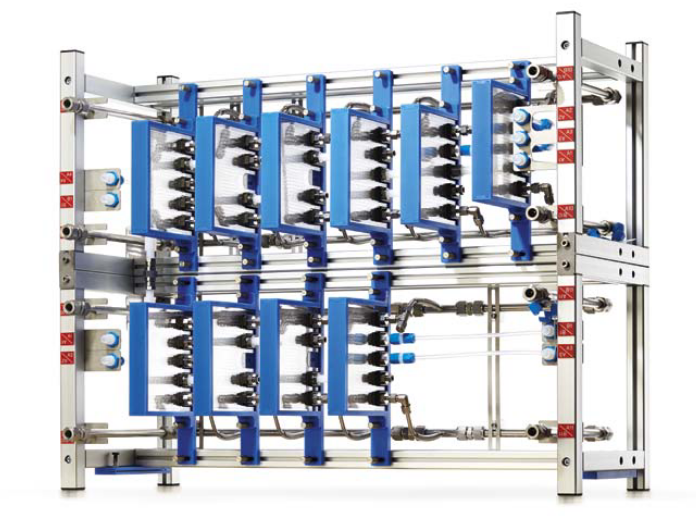
\includegraphics[scale=0.3]{reactor_example} }}%
	\qquad
	\subfloat[\centering micro flow element]{{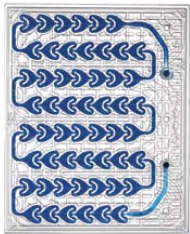
\includegraphics[scale=0.7]{reactor_element} }}%
	\caption{microfluidic system \cite{corning}}%
	\label{fig: reactor_examp}%
\end{figure}
Customization being not challenging by chaining different micro flow elements together, the industry can quickly adapt to upcoming new research or changing market environments.

Reactions taking place under these conditions are affected by Advection as a result of the moving fluid and diffusion as a result of concentration gradients. Therefor the hole moving system is called Reaction-Diffusion-Advection front or RDA front as an abbreviation.
These fronts play a significant role in a broad variety of technical and natural systems. They are applied, besides the already shown example from chemical engineering, in disease spreading \cite{kuto2017concentration}, population dynamics \cite{chen2018hopf, wang2019persistence} or biological applications \cite{zhao2011operator}. A common technical use case is the description of species distribution \cite{nakagaki1999reaction, von2013measurement}.

Until recently, the dynamics of fronts were studied for one-dimensional (1D) geometries \cite{PhysRevA.38.3151}. These 1D cases were carried out in a tubular system which is also a prominent reactor type within the industry. These studies were done for the chemical reaction $ A+B \rightarrow C$. This reaction is chosen because it is a simple reaction that can be investigated experimentally very well. The system contains only a forward reaction so the product that is build can be tracked. Ideally the reaction is a very fast one, so that the product is nearly instantly created where the species $A$ and $B$ meet. The developed approaches in tubes were later expanded and applied to cylindrical systems by Comolli, De Wit and Brau \cite{comolli2021dynamics}.

To gain further knowledge on how these pattern are build and how they develop over time theoretical models are needed. These models should describe the front dynamics from a cross-section point of view as this information can not be gained by experiments. 
\begin{figure}[htbp]
	\centering
	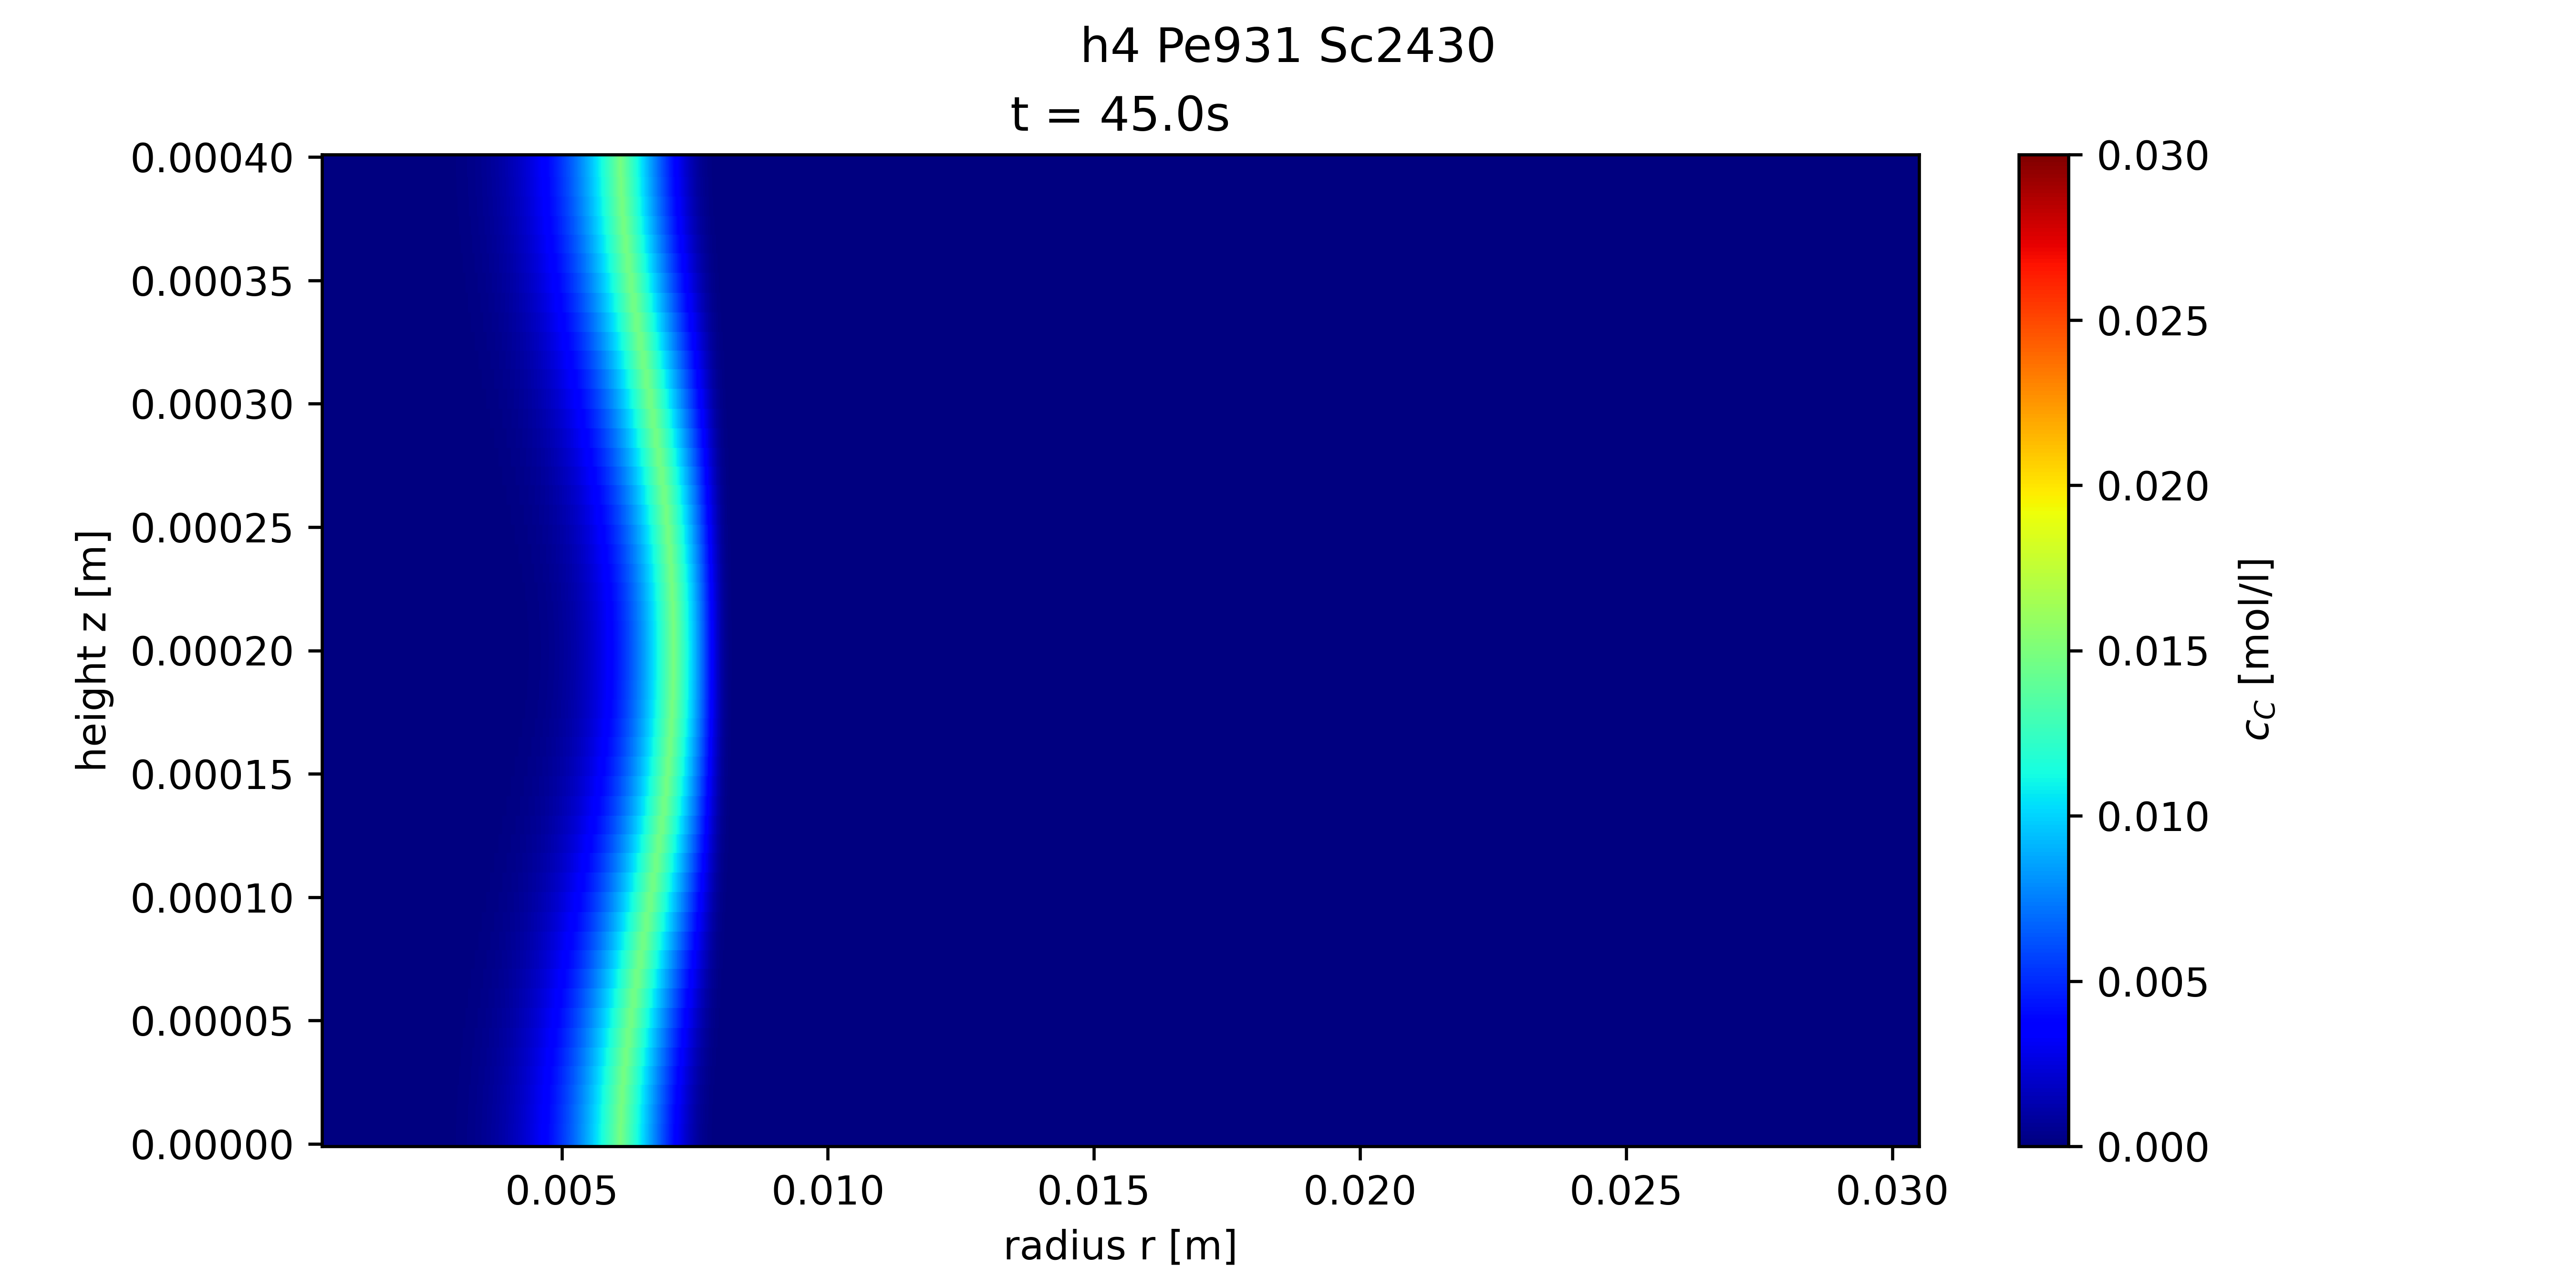
\includegraphics[scale=0.55]{front_example}
	\caption{RDA front example}
	\label{fig: front_example}
\end{figure}
As known from previous research the fronts curvature is dependent on the system's geometry and other input values. And example of such a front's appearance is shown in \autoref{fig: front_example}.

Within this work a model for the reaction-diffusion-advection system following the reaction $ A+B \rightarrow C$ is developed for a cylindrical geometry. Within this model the two initially separated species $A$ and $B$ are transported through advection and diffusion. $B$ is injected radially into $A$ from the cylinder's centreline. 

Special interest is in the species distribution at early stages of the developing reaction front. Experiments under $0g$ conditions have shown that some interesting patterns occur. The micro gravity experiments are needed because the two species are separating due to density differences resulting in an buoyancy effect as it can be schematically seen in \autoref{fig: 0g_example}.
\begin{figure}[htbp]
	\centering
	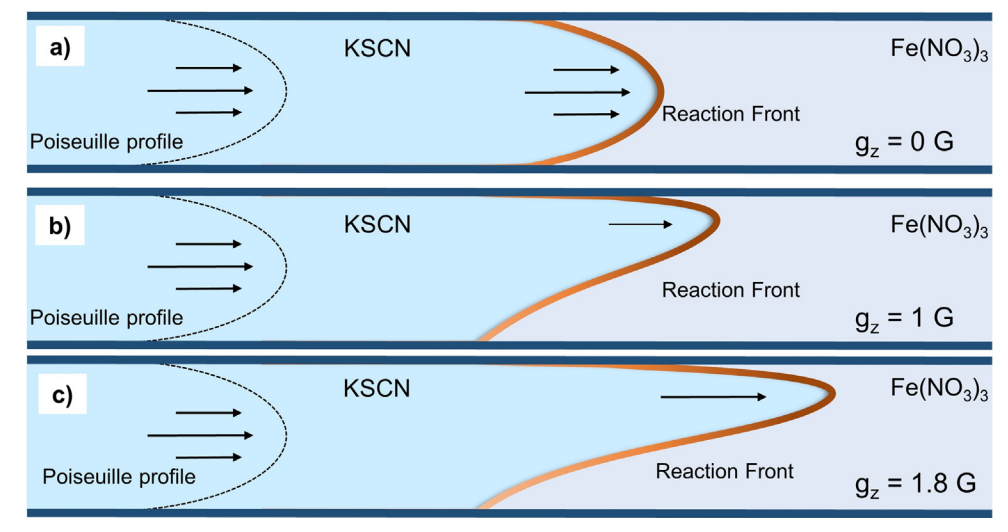
\includegraphics[scale=0.8]{0g_example}
	\caption{schematic of gravity effects on reaction fronts \cite{stergiou2022effects}}
	\label{fig: 0g_example}
\end{figure}
Within a model gravity can be turned off so investigations by changing geometric dimensions and other input values can be done more easily and quickly.

\section{objectives and report outline}

This work aims at the creation of a numerical model for a RDA front within a radial reactor using the modeling environment \texttt{Ansys FLUENT} \cite{manual2009ansys}. 

This work is divided into 6 sections. The theoretical background required for modelling is given in \autoref{chp:theory}. Following that the process of model creation is described in \autoref{chp:model}. Then in \autoref{chp:validation} the model's results are explained and compared against available experimental data. After the model validation the parametric studies results are shown and discussed within \autoref{chp:parameter_variation}. \autoref{chp:limitations} discusses limitations and error sources. Finally \autoref{chp:outlook} summarizes the work and provides an outlook for further use and improvements.

%In the end the created model can be generally applied and expanded to other geometries or more complex reactions to gain a deeper understanding of reaction-diffusion-advection fronts. 

% Was sind Peclet number und Schmidt number und welche Rolle spielen sie?, Sollte in der Motivation idealerwise schon auftauchen.


\end{document}